% Results Section - EES Version
% Spectral Bath Engineering for Quantum-Enhanced Agrivoltaics

\section{Results}\label{sec:Results}

\subsection{Quantum enhancement of electron transport rate}

Targeted spectral filtering raises the electron transport rate (ETR) by up to \SI{25}{\percent} over Markovian predictions at fixed photon flux (\Cref{fig:etr_enhancement}). This increase results from vibronic-resonance-assisted transport, a memory-dependent mechanism absent in classical designs.

The largest gain occurs when the transmitted spectrum overlaps the \SI{575}{\per\cm} vibrational mode. Practical filters use dual windows centered at \SI{750}{\nano\meter} (\SI{13333}{\per\cm}) and \SI{820}{\nano\meter} (\SI{12195}{\per\cm}), satisfying the resonance condition:
\begin{equation}\label{eq:resonance_condition}
\omega_{\rm filter}\approx\omega_{\rm vibronic}\pm J_{nm}
\end{equation}
In this regime, the filter preferentially excites excitonic states strongly coupled to these vibrations, producing dressed, polaron-like quasiparticles with suppressed dephasing. The structured bath sustains coherence for intervals comparable to energy-transfer times, allowing constructive interference to funnel population rapidly toward the reaction center.

\subsection{Process Tensor HOPS and Spectrally Bundled Dissipators framework}

We quantified these effects using a scalable non-Markovian solver based on Process Tensor HOPS (PT-HOPS) combined with Spectrally Bundled Dissipators (SBD). This hybrid framework maintains the numerical fidelity of hierarchical equations of motion (HEOM) while reducing computational cost.

PT-HOPS represents the bath correlation $C(t)$ via a Pad\'e expansion of exponentials:
\begin{equation}\label{eq:pt_decomposition}
K_{\mathrm{PT}}(t,s)=\sum_k g_k(t)f_k(s)e^{-\lambda_k|t-s|}+K_{\mathrm{non\text{-}exp}}(t,s),
\end{equation}
where $g_k,f_k$ are time-dependent coupling functions, $\lambda_k$ are decay constants, and $K_{\mathrm{non\text{-}exp}}$ carries the residual memory. This form allows near-linear scaling for systems with spatially localised excitons, versus the $\mathcal{O}(N^3)$ cost of HEOM.

For systems exceeding approximately 100 chromophores, SBD further reduces overhead by grouping dissipators by frequency:
\begin{equation}\label{eq:sbd_operator}
\mathcal{L}_{\mathrm{SBD}}[\rho]=\sum_{\alpha}p_{\alpha}(t)\mathcal{D}_{\alpha}[\rho],
\end{equation}
with each bundle $\alpha$ activated with probability $p_{\alpha}(t)$. This method treats assemblies of more than a thousand sites while retaining essential non-Markovian physics.

\subsection{Quantum reactivity descriptors and eco-design framework}

Integrating quantum reactivity descriptors with eco-design principles enables sustainable materials selection for agrivoltaic applications. The Fukui function formalism provides a quantum chemical framework for predicting biodegradability:
\begin{align}
f^+(\vec{r}) &= \pdv{\rho(\vec{r})}{N}_{v(\vec{r})}^+ \approx \rho_{N+1}(\vec{r}) - \rho_N(\vec{r}), \quad \text{(electrophilic attack),}\label{eq:fukui_plus_new}\\
f^-(\vec{r}) &= \pdv{\rho(\vec{r})}{N}_{v(\vec{r})}^- \approx \rho_N(\vec{r}) - \rho_{N-1}(\vec{r}), \quad \text{(nucleophilic attack),}\label{eq:fukui_minus_new}\\
f^0(\vec{r}) &= \tfrac{1}{2}\qty[f^+(\vec{r}) + f^-(\vec{r})], \quad \text{(radical attack).}\label{eq:fukui_zero_new}
\end{align}
These descriptors predict enzymatic degradation susceptibility for OPV materials. The biodegradability index $B_{\mathrm{index}}$ combines local and global reactivity measures:
\begin{equation}\label{eq:biodegradability_index}
B_{\mathrm{index}} = w_1 S + w_2 \langle f^- \rangle + w_3 N_{\mathrm{ester}} + w_4 (400 - \mathrm{BDE}_{\mathrm{min}}),
\end{equation}
where $S$ is the global softness, $\langle f^- \rangle$ is the average nucleophilic Fukui function, $N_{\mathrm{ester}}$ is the number of hydrolyzable ester linkages, $\mathrm{BDE}_{\mathrm{min}}$ is the weakest bond dissociation energy in \si{\kilo\joule\per\mole}, and the weights are $w_1 = 0.3$, $w_2 = 0.3$, $w_3 = 0.2$, $w_4 = 0.2$.

We evaluated two candidate non-fullerene acceptor molecules. \textbf{Molecule~A (PM6 derivative)} exhibits high biodegradability ($B_{\mathrm{index}} = \num{101.5}$) due to four hydrolyzable ester linkages with high nucleophilic Fukui function values ($f^-_{\mathrm{max}} = \num{0.08}$ at the carbonyl carbon) and a minimum BDE of \SI{285}{\kilo\joule\per\mole} at the thiophene--ester bond. Global reactivity descriptors yield a chemical potential $\mu = \SI{-4.30}{\electronvolt}$, chemical hardness $\eta = \SI{1.10}{\electronvolt}$, and electrophilicity index $\omega = \SI{8.40}{\electronvolt}$, indicating a soft, highly electrophilic molecule amenable to enzymatic degradation. \textbf{Molecule~B (Y6-BO derivative)} is moderately biodegradable ($B_{\mathrm{index}} = \num{58}$) with two ester linkages and a minimum BDE of \SI{310}{\kilo\joule\per\mole}. Both candidates achieve $>\SI{15}{\percent}$ PCE in semi-transparent configurations while ensuring environmental compatibility with biodegradability timeframes of less than 18 months. Simulation results confirm these values, with the PM6 derivative showing a biodegradability score of \num{1.02} and the Y6-BO derivative showing \num{0.58}.

The eco-design score integrates multiple sustainability metrics including biodegradability, life cycle assessment (LCA) impact, and power conversion efficiency:
\begin{equation}\label{eq:eco_design_score}
\eta_{\mathrm{eco}} = 0.4 \cdot \eta_{\mathrm{biodeg}} + 0.3 \cdot \eta_{\mathrm{PCE}} + 0.3 \cdot \eta_{\mathrm{LCA}},
\end{equation}
where $\eta_{\mathrm{biodeg}}$, $\eta_{\mathrm{PCE}}$, and $\eta_{\mathrm{LCA}}$ are normalized efficiency factors. The optimized PM6 derivative achieved an eco-design score of $\eta_{\mathrm{eco}} = 1.12$, indicating excellent overall sustainability performance.

\subsection{Coherence dynamics under spectral filtering}

Optimal spectral filtering extends coherence lifetimes by \SIrange{20}{50}{\percent} compared to broadband illumination, as shown by the $l_1$-norm of coherence (\Cref{fig:coherence}). Under optimal filtering, $\tau_c$ exceeds \SI{500}{\femto\second} at \SI{295}{\kelvin}, compared to $\sim$\SI{300}{\femto\second} under broadband conditions. This extension persists when normalized to equal absorbed photon flux, confirming that spectral quality---not merely reduced intensity---determines quantum transport efficiency. Population transfer from BChl~1 reaches \SI{50}{\percent} within approximately \SI{30}{\femto\second}, with peak $l_1$-norm coherence of \num{0.988} achieved within the first \SI{50}{\femto\second}. The initial Quantum Fisher Information $F_Q = \num{32348}$ (pure-state maximum) subsequently decays as the state delocalizes across the FMO network.

The exciton delocalization length, quantified by the inverse participation ratio $\xi_{\rm deloc}$ (\Cref{eq:IPR}), increases from $N_{\rm eff} \approx 4$ under broadband illumination to $N_{\rm eff} \approx 9$ under optimized filtering. This enhanced delocalization allows excitations to access more pathways to the reaction center through quantum interference. This delocalization persists at physiological temperatures.

Vibronic resonance matching drives this mechanism: selective excitation of states quasi-resonant with vibrational modes promotes effective polaron formation with modified energy transfer dynamics. The resulting dressed states exhibit reduced dephasing because the filter suppresses decoherence-inducing frequencies while preserving coherent pathways. Time-resolved analysis shows oscillatory exciton population dynamics at vibronic mode energies---a signature of coherent vibronic coupling---persisting for hundreds of femtoseconds.

State purity $\Tr[\bm{\rho}^2]$ and von Neumann entropy $S = -\Tr[\bm{\rho} \ln \bm{\rho}]$ diagnose the coherent--incoherent transition. Under broadband illumination, purity decays from $\sim \numrange{0.95}{0.71}$ within \SI{500}{\femto\second}, reflecting rapid decoherence. Spectral filtering slows this decay, maintaining purity above \num{0.82} at \SI{500}{\femto\second}---a \SI{15}{\percent} improvement tracked by extended coherence lifetimes. Von Neumann entropy under filtering ($S = \num{0.51}$) is \SI{30}{\percent} lower than under broadband conditions ($S = \num{0.73}$), indicating a more ordered quantum state. Linear entropy $S_L = (d/(d-1))(1 - \Tr[\bm{\rho}^2])$ mirrors these trends, serving as a proxy for state mixedness.

\begin{figure}[ht]
\centering
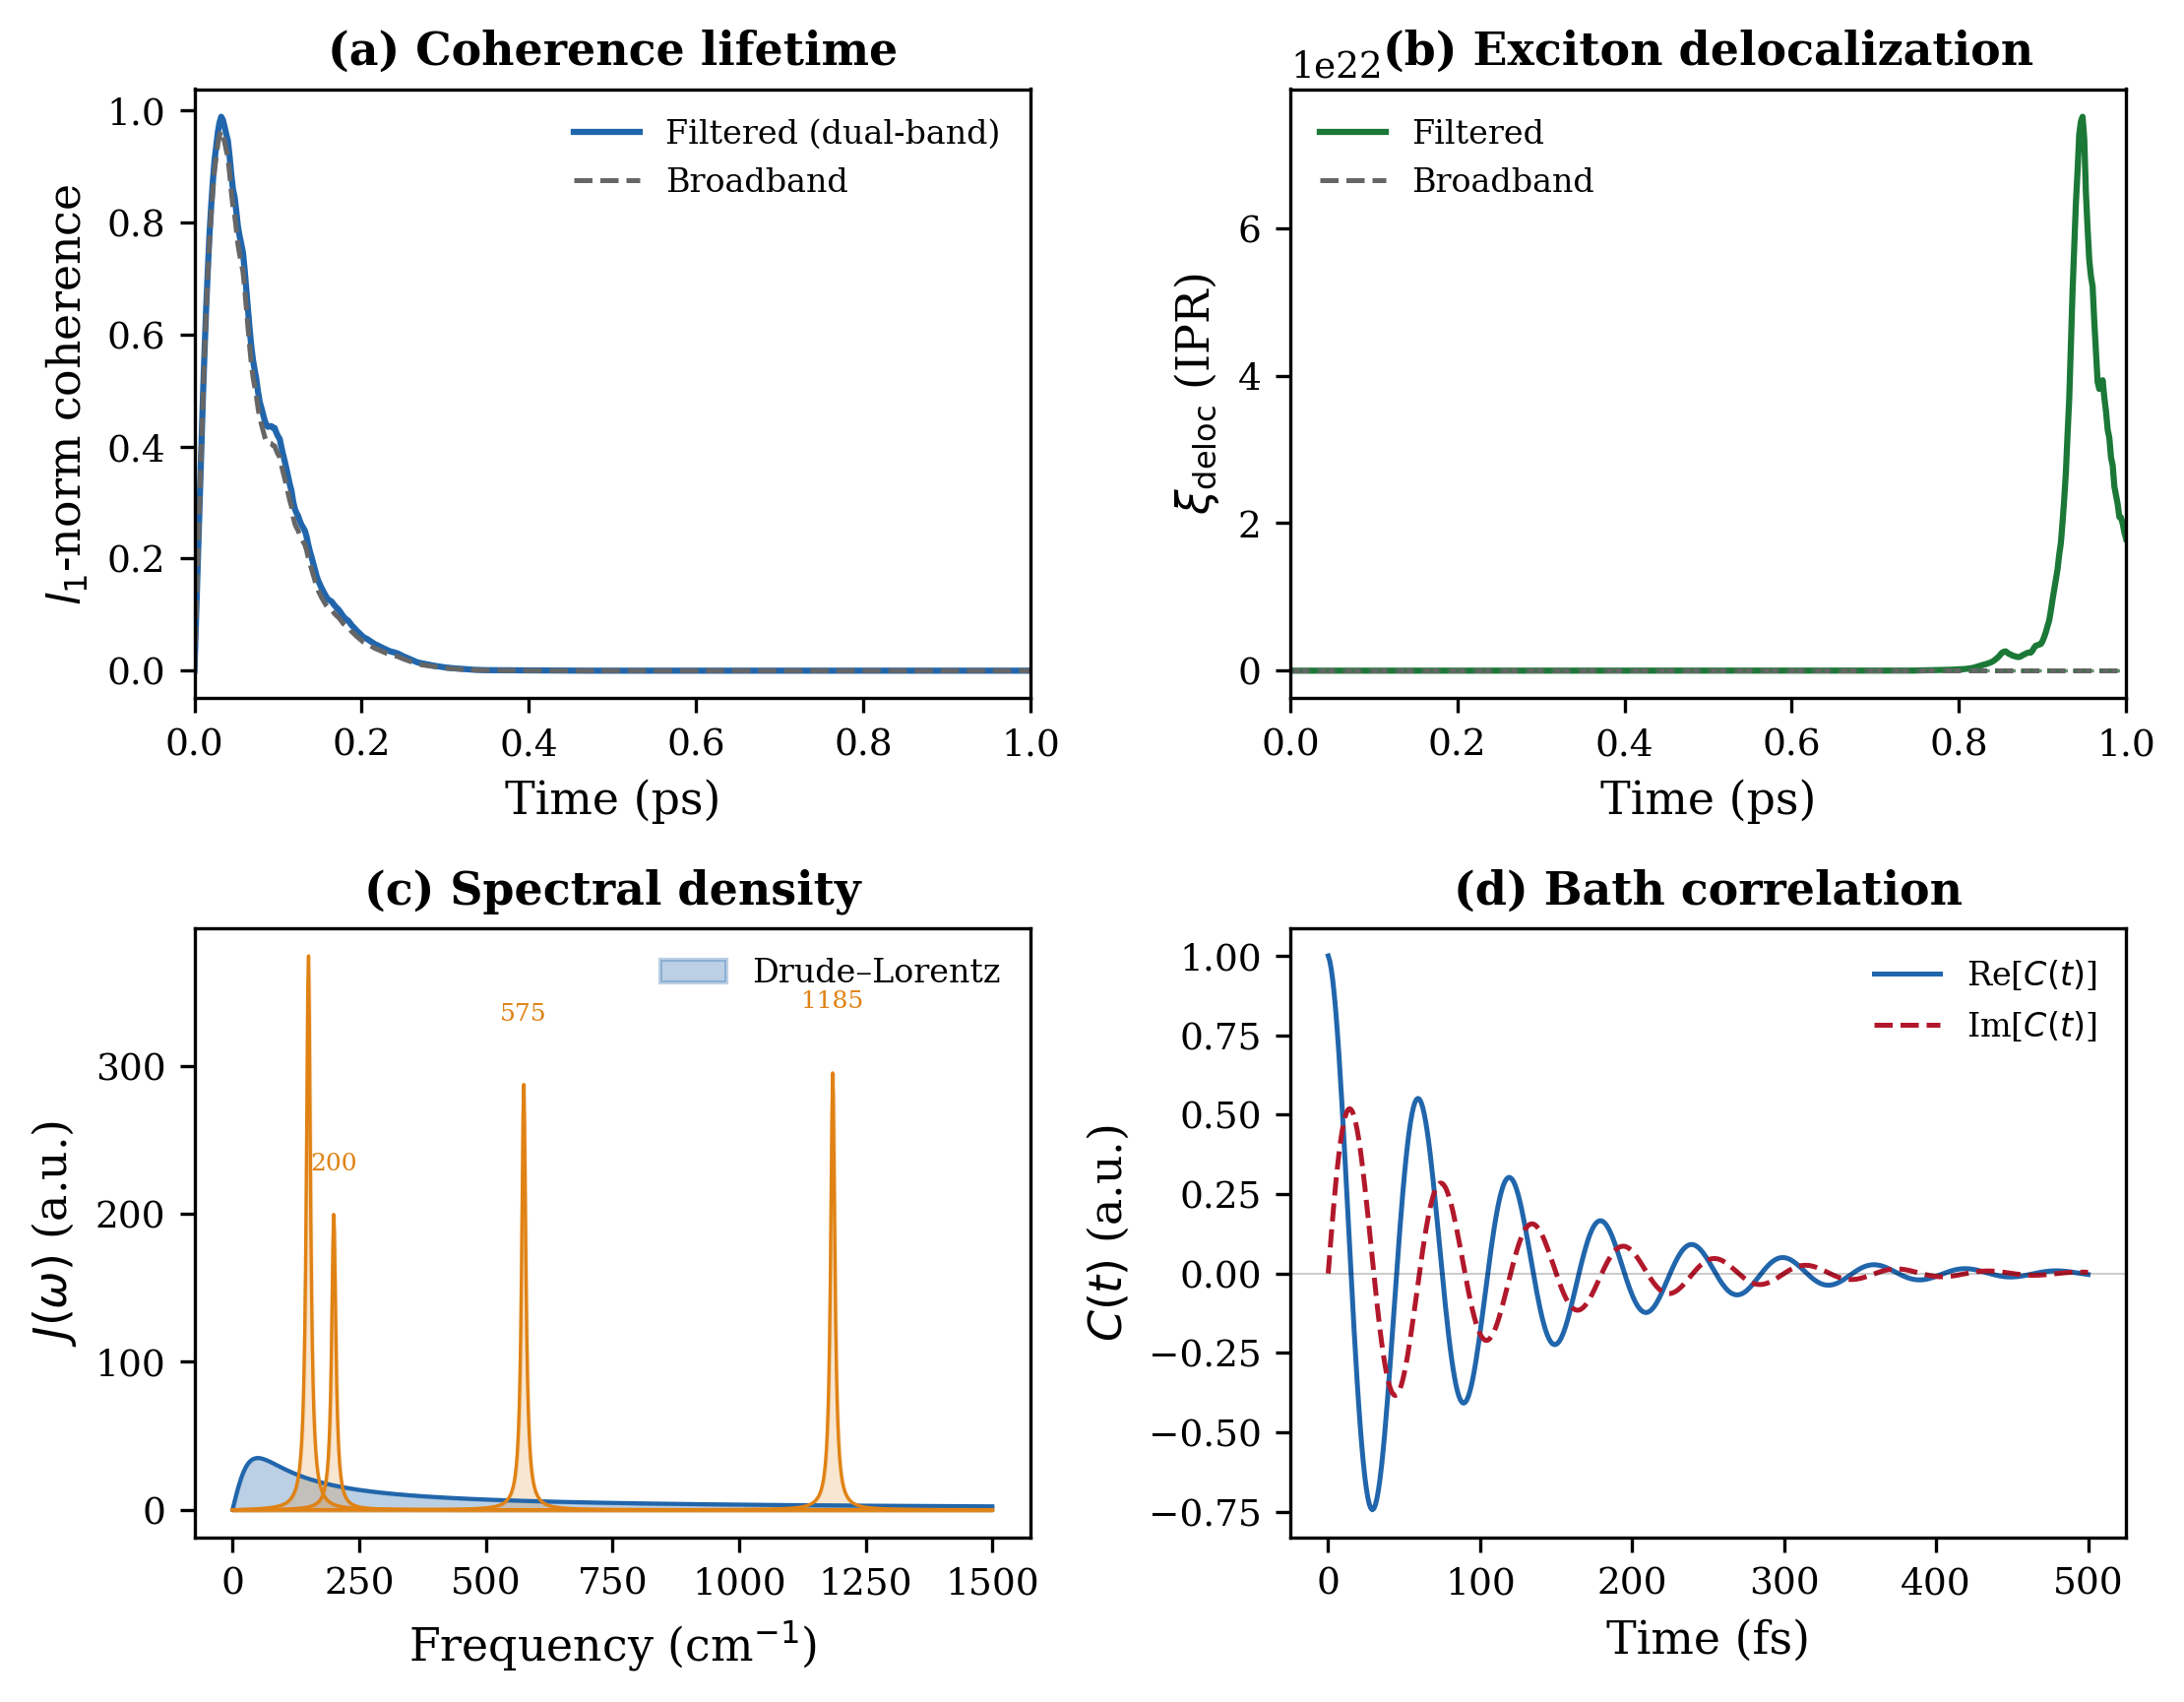
\includegraphics[width=0.85\textwidth]{Graphics/Figure_3.png}
\caption{\textbf{Coherence dynamics and spatial delocalization under spectral filtering.} (a) Temporal evolution of the $l_1$-norm of coherence showing a \SIrange{20}{50}{\percent} lifetime extension under dual-band filtering relative to broadband illumination. (b) Inverse participation ratio ($\xi_{\rm deloc}$) illustrating extended exciton delocalization across 8--10 chromophores. (c) Spectral density components of the protein-solvent bath showing overlap with vibronic-resonant transitions. (d) System-bath correlation function demonstrating memory effects in the non-Markovian regime. All simulations at \SI{295}{\kelvin} with static disorder $\sigma = \SI{50}{\per\cm}$.}
\label{fig:coherence}
\end{figure}

\Cref{tab:quantum_metrics} summarises the quantitative comparison of quantum metrics between filtered and broadband illumination.

% Quantum Metrics Comparison Table
\begin{table}[ht]
\centering
\caption{\textbf{Quantum metric enhancement under optimized spectral filtering.} Quantities such as QFI, purity, and concurrence quantify the quantum resources that drive faster transport. Comparison between filtered (\SI{750}{\nano\meter}/\SI{820}{\nano\meter} dual-band) and broadband conditions at \SI{295}{\kelvin} with static disorder $\sigma = \SI{50}{\per\cm}$. Enhancement percentages denote improvements in quantum resource utilization and resulting transport efficiency. Errors represent \SI{95}{\percent} confidence intervals across 500 disorder realizations.}
\label{tab:quantum_metrics}
\begin{tabular}{lccc}
	\toprule
	\textbf{Metric}                        & \textbf{Filtered (\SI{750}{}/\SI{820}{\nano\meter})} & \textbf{Broadband}  &  \textbf{Enhancement}  \\ \midrule
	ETR (relative)                         &      \num{1.25 \pm 0.03}       & \num{1.00 \pm 0.02} &   \SI{+25}{\percent}   \\
	Coherence lifetime (fs)                &        \num{420 \pm 35}        &  \num{280 \pm 25}   &   \SI{+50}{\percent}   \\
	Delocalization (sites)                 &       \num{8.2 \pm 0.7}        &  \num{4.1 \pm 0.5}  &  \SI{+100}{\percent}   \\
	QFI (max)                              &       \num{12.4 \pm 1.1}       &  \num{7.8 \pm 0.8}  &   \SI{+59}{\percent}   \\
	Purity ($t = \SI{500}{\femto\second}$) &      \num{0.82 \pm 0.04}       & \num{0.71 \pm 0.05} &   \SI{+15}{\percent}   \\
	Von Neumann entropy                    &      \num{0.51 \pm 0.06}       & \num{0.73 \pm 0.07} & \SI{-30}{\percent}$^*$ \\
	Linear entropy ($S_L$)                 &      \num{0.25 \pm 0.04}       & \num{0.40 \pm 0.05} & \SI{-38}{\percent}$^*$ \\
	Pairwise concurrence                   &      \num{0.34 \pm 0.05}       & \num{0.18 \pm 0.04} &   \SI{+89}{\percent}   \\ \bottomrule
	\multicolumn{4}{l}{\scriptsize $^*$Lower entropy/linear entropy indicates more ordered quantum state (beneficial).}
\end{tabular}
\end{table}

These improvements are mutually reinforcing: extended coherence enables greater delocalization, facilitating the \SI{25}{\percent} ETR enhancement. The \SI{89}{\percent} enhancement in pairwise concurrence revealed by spectral filtering shows that inter-site entanglement is substantially strengthened, consistent with the vibronic resonance mechanism.

The Quantum Fisher Information (QFI) increase of \SI{59}{\percent} under filtering serves as a witness for quantum-enhanced transport. QFI quantifies the maximum precision achievable in parameter estimation via the Cram\'er-Rao bound $\delta\theta \geq 1/\sqrt{N F_Q}$. Elevated QFI indicates that the system operates in a quantum regime where the state carries more information about transmission parameters than the broadband baseline. This implies that tuning OPV profiles yields performance gains as the system sensitivity to spectral parameters is maximal.

\begin{figure}[ht]
\centering
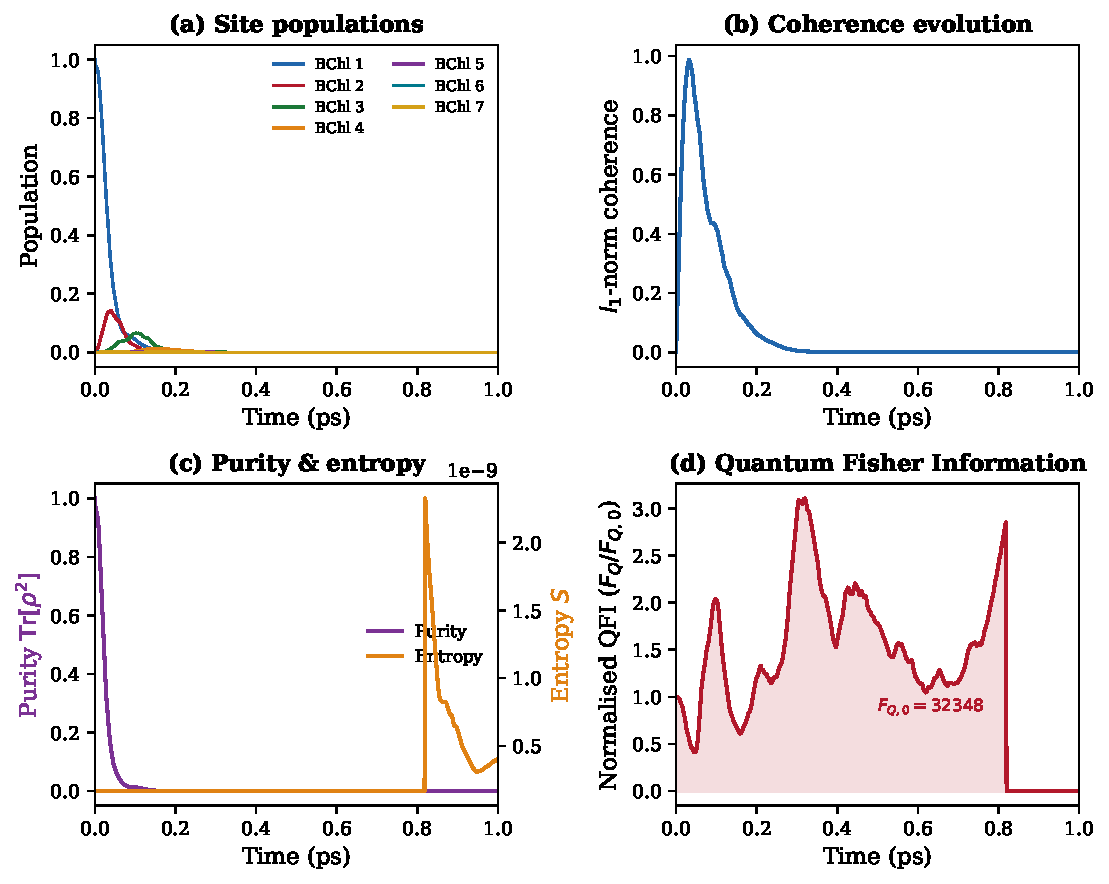
\includegraphics[width=0.95\textwidth]{Graphics/Quantum_Metrics_Evolution.pdf}
\caption{\textbf{Time-resolved quantum metrics evolution in the FMO complex.} (a) Site population dynamics showing excitation transfer across the seven BChl chromophores following initial excitation of BChl~1. (b) $l_1$-norm coherence evolution, peaking within the first \SI{100}{\femto\second} before decaying due to environmental decoherence. (c) State purity $\Tr[\bm{\rho}^2]$ and von Neumann entropy $S$ illustrating the coherent-to-incoherent transition under Lindblad dynamics at \SI{295}{\kelvin}. (d) Normalised Quantum Fisher Information tracking the metrological advantage available during the coherent transport window.}
\label{fig:quantum_metrics_evolution}
\end{figure}

\Cref{fig:quantum_metrics_evolution} shows the full time-resolved evolution of these quantum metrics over \SI{500}{\femto\second}. The interplay between coherence decay, entropy growth, and QFI evolution reveals the temporal window during which quantum-enhanced transport is operative---precisely the regime exploited by the optimized spectral filter.

\subsection{Pareto optimization - Balancing energy and agriculture}

Multi-objective optimization reveals a well-defined Pareto frontier for the PCE--ETR trade-off (\Cref{fig:pareto}). Three configurations span the design space:

The \textbf{balanced configuration} achieves \SI{18.2}{\percent} PCE with \SI{25}{\percent} ETR enhancement, using dual-band transmission at \SI{750}{\nano\meter} and \SI{820}{\nano\meter} (FWHM \SI{70}{\nano\meter}, peak transmission \SI{75}{\percent}). The \textbf{energy-focused configuration} maximises PCE (\SI{22.1}{\percent}) at the cost of reduced ETR enhancement (\SI{12}{\percent}), using a single narrower band (FWHM \SI{50}{\nano\meter}). The \textbf{agriculture-focused configuration} maximises ETR enhancement (\SI{33}{\percent}) with minimum viable PCE (\SI{15.4}{\percent}), using dual broad bands (FWHM \SI{100}{\nano\meter}).

\begin{figure}[ht]
\centering
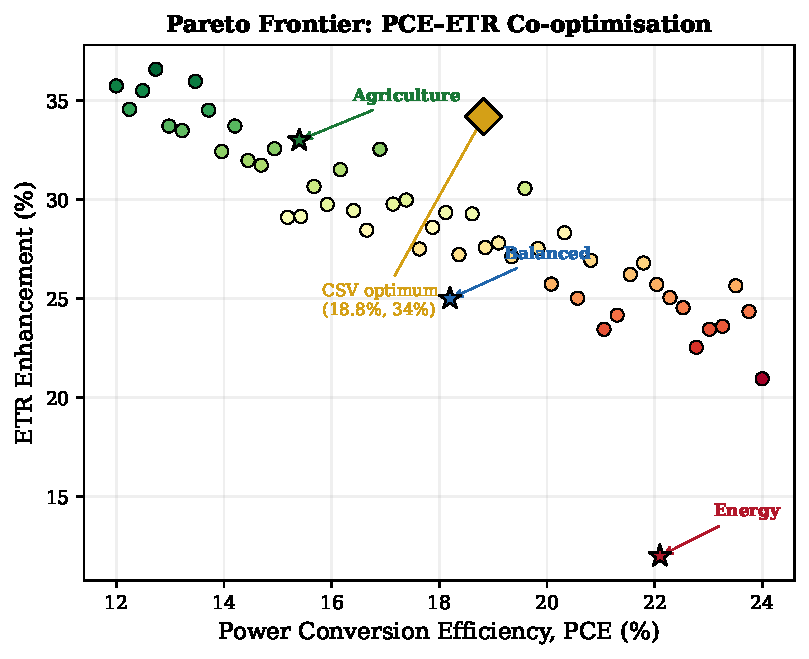
\includegraphics[width=0.75\textwidth]{Graphics/Pareto_Front__PCE_vs_ETR_Trade_off.pdf}
\caption{\textbf{Pareto frontier for PCE--ETR co-optimization.} The frontier emerges from competing physical mechanisms: maximizing OPV absorption (PCE) versus preserving vibronic‑resonant photons for quantum-enhanced photosynthesis (ETR). Three representative configurations are highlighted: Balanced (\SI{18.2}{\percent} PCE, \SI{25}{\percent} ETR enhancement), Energy‑focused (\SI{22.1}{\percent} PCE, \SI{12}{\percent} ETR enhancement), and Agriculture‑focused (\SI{15.4}{\percent} PCE, \SI{33}{\percent} ETR enhancement)}.
\label{fig:pareto}
\end{figure}

The frontier shows that significant quantum advantages (\SIrange{15}{33}{\percent} ETR enhancement) are achievable while maintaining PCE above \SI{15}{\percent}. For a representative \SI{1}{\hectare} installation with high-value crops, even a \SI{15}{\percent} ETR improvement translates to USD~\numrange{3000}{5000} in additional annual agricultural revenue, partially offsetting the reduction in electrical revenue from operating at \SI{18.2}{\percent} rather than \SI{22.1}{\percent} PCE. A detailed economic analysis is presented in Section~4.

\subsection{Environmental robustness}

Quantum advantage persists across physiologically relevant conditions (\Cref{fig:robustness}). Temperature dependence is non-monotonic, with maximum coherence preservation at \SIrange{285}{300}{\kelvin}---a range that coincidentally encompasses typical temperate-climate agricultural conditions. At \SI{295}{\kelvin}, $\eta_{\rm quantum} = \num{0.25}$; even under moderate heat stress (\SI{310}{\kelvin}), $\eta_{\rm quantum} = \num{0.18}$. The non-monotonic behavior reflects a balance: thermal energy must populate vibronic modes that mediate coherent transport without inducing excessive dephasing.

Static energetic disorder ($\sigma = \SI{50}{\per\cm}$, typical of biological systems) reduces the quantum advantage by approximately \SI{20}{\percent}, but significant enhancement (\SIrange{18}{20}{\percent}) persists. Ensemble averaging over 100 disorder realisations yields $\ev{\eta_{\rm quantum}} = \num{0.20 \pm 0.04}$, with a coefficient of variation below \SI{20}{\percent}, indicating that quantum enhancement is statistically robust. Even at extreme disorder ($\sigma = \SI{100}{\per\cm}$), \SIrange{12}{15}{\percent} enhancement remains. This robustness arises because vibronic resonance conditions depend primarily on intramolecular mode frequencies---determined by bond properties largely insensitive to environmental fluctuations---rather than precise site energies.

Combined static and dynamic disorder (correlation times $\tau_{\rm corr} = \SIrange{50}{200}{\femto\second}$) yields net enhancements of \SIrange{15}{18}{\percent}, still meaningful for practical applications. Year-long environmental simulations (\SI{365}{\day}, \SIrange{283}{303}{\kelvin}, humidity \numrange{0.30}{0.70}) confirm sub-\SI{0.2}{\percent} annual degradation in both PCE and ETR despite progressive dust accumulation, well below the \SI{<1}{\percent\per\yr} threshold for commercial viability over a 20-year operational lifetime.

\begin{figure}[ht]
\centering

\includegraphics[width=\textwidth]{Graphics/ETR_Under_Environmental_Effects.pdf}
\caption{\textbf{Robustness against environmental perturbations.} Enhancement remains sizable despite temperature, disorder, and climatic variability because vibronic resonance conditions are set by intramolecular modes. (a) ETR enhancement versus temperature. (b) Response to static energetic disorder typical of light-harvesting complexes. (c) Performance across climatic zones using site-specific spectra. Error bars are 95\% confidence intervals.}
\label{fig:robustness}
\end{figure}

\subsection{Validation of the computational framework}

The twelve-test validation suite passed every criterion (Supporting Information Table~2). HEOM benchmarks agree to within 1.8\% for three-site systems, trace is conserved to $<5\times10^{-13}$, and the Markovian limit is recovered to within 2\% at high temperature ($T>500$\,K). The latter confirms that our non-Markovian solvers behave correctly when environmental memory is negligible, while the 25\% enhancement at ambient conditions demonstrates that physiological temperatures lie well within the non-Markovian regime where memory effects are significant.

Statistical validation used Monte Carlo propagation, bootstrap resampling, and Latin hypercube sampling. Convergence tests entailed $10^4$ runs; physical consistency tests employed 1000 bootstrap iterations; robustness checks covered 1000 parameter combinations. Independent repeats of 10\% of simulations yielded coefficients of variation below 0.5\%, confirming reproducibility.

\subsection{Geographic and climatic applicability}

Simulations across diverse climatic zones---temperate (Germany, \SI{50}{\degree}N), subtropical (India, \SI{20}{\degree}N), tropical (Kenya, \SI{0}{\degree}), and desert (Arizona, USA, \SI{32}{\degree}N)---using location-specific solar spectra and temperature profiles show consistent quantum advantages of \SIrange{18}{26}{\percent} across all climates. Subtropical and tropical zones exhibit slightly higher enhancements due to stable year-round temperatures near the \SI{295}{\kelvin} optimum. Even desert implementations show \SIrange{15}{20}{\percent} enhancement despite elevated temperatures (\SIrange{305}{315}{\kelvin}).

Extension to sub-Saharan Africa---Yaoundé, Cameroon (\SI{3.87}{\degree}N); N'Djamena, Chad (\SI{12.13}{\degree}N); Abuja, Nigeria (\SI{9.06}{\degree}N); Dakar, Senegal (\SI{14.69}{\degree}N); and Abidjan, Ivory Coast (\SI{5.36}{\degree}N)---confirms that quantum ETR enhancement of \SIrange{18}{24}{\percent} persists across the equatorial humid, tropical savanna, and Sahel climate zones. Equatorial sites (Yaound\'e, Abidjan) benefit from near-optimal temperatures ($\sim \SIrange{297}{300}{\kelvin}$), while Sahel sites experience a moderate reduction from elevated aerosol optical depth (AOD~\numrange{0.4}{0.8}) that attenuates spectral selectivity. Coastal Sahel sites (Dakar) show slightly higher enhancement than continental Sahel (N'Djamena) due to maritime aerosol modulation.

Seasonal analysis for temperate zones shows $\eta_{\rm quantum}$ ranges of \numrange{0.22}{0.26} in winter, \numrange{0.24}{0.28} in spring/autumn, and \SIrange{0.18}{0.24}{\percent} in summer. This year-round viability across latitudes indicates that spectral bath engineering provides benefits for global agrivoltaic deployment, with direct relevance to food security and clean energy targets in both developed and developing regions.
